\documentclass[english, 11 pt, class=article, crop=false]{standalone}
%\documentclass[english, 11 pt]{report}
\usepackage[T1]{fontenc}
\usepackage[utf8]{luainputenc}
\usepackage{babel}
\usepackage[hidelinks, bookmarks]{hyperref}
\usepackage{geometry}
\geometry{verbose,tmargin=1cm,bmargin=3cm,lmargin=4cm,rmargin=4cm,headheight=3cm,headsep=1cm,footskip=1cm}
\setlength{\parindent}{0bp}
\usepackage{amsmath}
\usepackage{amssymb}
\usepackage{esint}
\usepackage{import}
\usepackage[subpreambles=false]{standalone}
%\makeatletter
\addto\captionsenglish{\renewcommand{\chaptername}{Kapittel}}
\makeatother
\usepackage{tocloft}
\addto\captionsenglish{\renewcommand{\contentsname}{Innhold}}
\usepackage{graphicx}
\usepackage{placeins}
\raggedbottom
\usepackage{calc}
\usepackage{cancel}
\makeatletter
\usepackage{color}
\definecolor{shadecolor}{rgb}{0.105469, 0.613281, 1}
\usepackage{framed}
\usepackage{wrapfig}
\usepackage{bm}
\usepackage{ntheorem}

\usepackage{ragged2e}
\RaggedRight
\raggedbottom
\frenchspacing

\newcounter{lign}[section]
\newenvironment{lign}[1][]{\Large \refstepcounter{lign} \large
	\textbf{\thelign #1} \rmfamily}{\par\medskip}
\numberwithin{lign}{section}
\numberwithin{equation}{section}
\usepackage{xcolor}
\usepackage{icomma}
\usepackage{mathtools}
\usepackage{lmodern} % load a font with all the characters
\usepackage{xr-hyper}
\makeatother
\usepackage[many]{tcolorbox}

%\setlength{\parskip}{\medskipamount}
\newcommand{\parskiplength}{11pt}
%\setlength{\parskip}{0 pt}
\newcommand\eks[2][]{\begin{tcolorbox}[enhanced jigsaw,boxrule=0.3 mm, arc=0mm,breakable,colback=green!30] {\large \textbf{Eksempel #1} \vspace{\parskiplength}\\} #2 \vspace{1pt} \end{tcolorbox}\vspace{1pt}}

\newcommand\fref[2][]{\hyperref[#2]{\textsl{Figur \ref*{#2}#1}}}
\newcommand{\hr}[2]{\hyperref[#2]{\color{blue}\textsl{#1}}}

\newcommand\rgg[2][]{\begin{tcolorbox}[boxrule=0.3 mm, arc=0mm,colback=orange!55] #2 \vspace{1pt} \end{tcolorbox}\vspace{-2pt}}
\newcommand\alg[1]{\begin{align*} #1 \end{align*}}
\newcommand\algv[1]{\vspace{-11 pt} \begin{align*} #1 \end{align*}}
\newcommand\vs{\vspace{-11 pt}}
\newcommand\g[1]{\begin{center} {\tt #1}  \end{center}}
\newcommand\gv[1]{\begin{center} \vspace{-22 pt} {\tt #1} \vspace{-11 pt} \end{center}}
%\addto\captionsenglish{\renewcommand{\contentsname}{Løsningsforslag tentamen R2 H2015}}

% Farger
\colorlet{shadecolor}{blue!30} 

% Figur
\usepackage{float}
\usepackage{subfig}
\captionsetup[subfigure]{labelformat=empty}
\usepackage{esvect}

\newcommand\sv{\textbf{Svar:} \vspace{5 pt} \\}

%Tableofconents
\renewcommand{\cfttoctitlefont}{\Large\bfseries}
\setlength{\cftsubsecindent}{2 cm}
\newcommand\tocskip{6 pt}
\setlength{\cftaftertoctitleskip}{30 pt}
\setlength{\cftbeforesecskip}{\tocskip}
%\setlength{\cftbeforesubsecskip}{\tocskip}

%Footnote:
\usepackage[bottom, hang, flushmargin]{footmisc}
\usepackage{perpage} 
\MakePerPage{footnote}
\addtolength{\footnotesep}{2mm}
\renewcommand{\thefootnote}{\arabic{footnote}}
\renewcommand\footnoterule{\rule{\linewidth}{0.4pt}}

%asin, atan, acos
\DeclareMathOperator{\atan}{atan}
\DeclareMathOperator{\acos}{acos}
\DeclareMathOperator{\asin}{asin}

%Tabell
\addto\captionsenglish{\renewcommand{\tablename}{Figur}}

% Figur
\usepackage[font=footnotesize,labelfont=sl]{caption}
\addto\captionsenglish{\renewcommand{\figurename}{Figur}}

% Figurer
\newcommand\scr[1]{/home/sindre/R/scr/#1}
\newcommand\asym[1]{/home/sindre/R/asymptote/#1}

%Toc for seksjoner
\newcommand\tsec[1]{\phantomsection\addcontentsline{toc}{section}{#1}
	\section*{#1}}
%\newcommand\tssec[1]{\subsection*{#1}\addcontentsline{toc}{subsection}{#1}}
\newcommand\tssec[1]{\subsection*{#1}}
% GeoGebra
\newcommand{\cms}[2]{{\tt #1( #2 )}}
\newcommand{\cm}[2]{{\large \tt #1( #2 )} \gvs \\}
\newcommand{\cmc}[2]{{\large \tt #1( #2 )} \large (CAS)  \gvs \\ \normalsize}
\newcommand{\cmk}[2]{{\large \tt #1( #2 )} \large (Inntastingsfelt)  \gvs \\ \normalsize}

\newcommand\gvs{\vspace{11 pt}}

\newcommand\vsk{\vspace{11 pt}}
\newcommand{\merk}{\vsk \textsl{Merk}: }
\newcommand{\fig}[1]{
\begin{figure}
	\centering
	\includegraphics[scale=0.5]{fig/#1}
\end{figure}
}
\newcommand{\figc}[1]{
		\centering
		\includegraphics[scale=0.5]{fig/#1}
}

% Opg
%\newcommand{\opgt}{\phantomsection \addcontentsline{toc}{section}{Oppgaver} \section*{Oppgaver for kapittel \thechapter}}
\newcounter{opg}
\numberwithin{opg}{section}

\newcommand{\opl}[1]{\vspace{15pt} \refstepcounter{opg} \textbf{\theopg} \vspace{2 pt} \label{#1} \\}



\begin{document}
\eqlen
\opgt
\setcounter{section}{1}	
\opl{udir}
Utdanninsdirektoratet definerer størrelsen til en vinkel $ v $ mellom to linjestykker $ a $ og $ b $, oppgitt i radianer,  på følgende måte:\os

\textsl{Forholdet mellom lengden på en bue mellom $ a $ og $ b $ og radiusen til buen.}
\begin{figure}
	\centering
	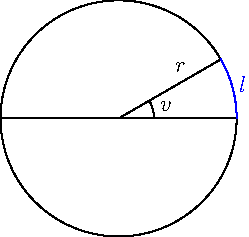
\includegraphics[]{../../asymptote/rad}
\end{figure}
I figuren over svarer dette til forholdet $ \dfrac{l}{r} $.
\os
Forklar hvorfor radianer ut ifra denne definisjonen også kan sees på som en buelengde langs enhetssirkelen.

\opl{rads}
Gjør om til radianer:\os
\begin{tabular}{@{}l l}
	\textbf{a)} $ 60^\circ $ & \quad \textbf{b)} $ 15^\circ $
\end{tabular}

\opl{grad}
Gjør om til grader:\os

\begin{tabular}{@{}l l}
	\textbf{a)} $ \dfrac{11\pi}{12} $ & \quad \textbf{b)} $ \dfrac{11\pi}{6} $
\end{tabular}

\nes
\opl{pytg}
Bruk Pytagoras' setning og definisjonen av $ \cos x $ og $ \sin x $ til å vise at
\[ \cos^2 x + \sin^2 x = 1 \] 

\opl{tanx}
Finn $\tan x $ når du vet at\\
\begin{tabular}{@{}l l}
	\textbf{a)} $ \sin x = 0$ og $ \cos x=1 $ & \quad \textbf{b)} $ \sin x = \dfrac{1}{2} $ og $ \cos x = -\dfrac{\sqrt{3}}{2} $
\end{tabular}
\newpage
\opl{kvadrant}
Bruk $ - $ og $ + $ for å indikere henholdsvis negativ og positiv, og sett riktige markører i tabellen under.\os

\begin{tabular}{@{}l|l| l| l|l|}
&1. kvadrant & 2. kvadrant & 3. kvadrant & 4. kvadrant\\ \hline
$ \sin x $& & & &\\ \hline
$ \cos x $& & & &\\ \hline
$ \tan x $& & & &\\\hline
\end{tabular}

\opl{trigverd}
Bestem verdien til\os
\begin{tabular}{@{}l l l l }
\textbf{a)} $ \sin\left(-\frac{\pi}{6}\right) $ &\quad \textbf{b)} $ \cos \pi $ &\quad \textbf{c)} $ \cos\left(-\frac{\pi}{2}\right) $&\quad \textbf{d)} $ \tan\left(\frac{2\pi}{3}\right) $
\end{tabular}

\opl{averdier}
Finn verdien til\\ \renewcommand{\arraystretch}{1.7}
\begin{tabular}{@{}l l l l }	
\textbf{a)} $ \asin 0 $ &\quad\textbf{b)} $ \asin \frac{\sqrt{3}}{2} $ \\
 \textbf{c)} $ \acos (-1) $ &\quad\textbf{d)} $ \acos \left(-\frac{\sqrt{2}}{2}\right) $ \\
 \textbf{e)} $ \atan 1 $ &\quad\textbf{f)} $ \atan \left(\frac{1}{\sqrt{3}}\right) $
\end{tabular}\renewcommand{\arraystretch}{1}

\opl{bruk1}
Bruk \eqref{1} til å vise at $ {\sin\left(\frac{\pi}{6}\right)=\frac{1}{2}} $ når du vet at $ \cos\left(\frac{\pi}{6}\right)=\frac{\sqrt{3}}{2} $.

\opl{sin2xopg}
\textbf{a)} Bruk én av de trigonometriske identitetene til å vise at
\[  \sin (2x)=2\cos x\sin x \]
\textbf{b)} Gitt at $ {\sin \left(\frac{\pi}{6}\right)=\frac{1}{2}} $. Bruk dette og identiteten over til å vise at
\[ 2\cos \left(\frac{\pi}{12}\right)\sin \left(\frac{\pi}{12}\right) = \frac{1}{2} \]

\opl{cossomsin}
Skriv om utrykket
\[ \cos \left(3x-\frac{5\pi}{2}\right) \]
til et sinusuttrykk.
\newpage
\opl{cossinsin}
Skriv om uttrykket \[ \cos( 2x) + \sqrt 3\sin (2x) \]
til et sinusuttrykk.

\nes

\opl{sincos0}
Vis at alle løsninger av ligningen $ \cos x=0 $ er gitt som
\[ x = \frac{\pi}{2}+\pi n \]
mens alle løsninger av ligningen $ \sin x = 0 $ er gitt som
\[ x = \pi n \]\vds \vs

\opl{triligns}
Løs ligningene:\os

\textbf{a)} $ \cos x=\frac{\sqrt{2}}{2} $\os

\textbf{b)} $ \cos \left(\frac{\pi}{3}x\right) = 0\quad,\quad x\in[0, 5]$\os

\textbf{c)} $ 2\sin(3x)=1 $\os

\textbf{d)} $ \sin(2x-\pi)=-\frac{\sqrt{3}}{2} $\os

\textbf{e)} $ 2\sqrt{3}\tan \left(4x+\frac{\pi}{2}\right) = 2$ \os

\opl{asinbcos0o}
Løs ligningene:\os

\textbf{a)} $\sqrt{3} \sin x - \cos x =0$\os

\textbf{b)} $ \sin x + \sqrt{3}\cos x =0$\os

\textbf{c)} $ \cos (2x) + \sin (2x)=0  $\os


\opl{kombo}
Løs ligningene:\os
\textbf{a)} $ \cos x - \sin x = \sqrt{2}  $ \os

\textbf{b)} $ \sqrt{3} \cos\left(\dfrac{x}{2\pi}\right) - \sin\left(\dfrac{x}{2\pi}\right)=1 $\os
\nes
\newpage
\opl{abctri}
Løs ligningene:\os
\textbf{a)} $ \sin^2 x+\frac{1}{2}\sin x-\frac{1}{2}=0 $\os

\textbf{b)} $ \cos^2 (3x) -3\cos (3x) -4=0$\os

\textbf{c)} $ 2\cos^2 x+ \sqrt{8} \cos x+1=0 $\os

\textbf{d)} $ \tan^2 (\pi x) -\sqrt{12}\tan (\pi x) +  3=0$\os

\textbf{e)} $ -\sin^2(3x)- 3\cos (3x) -3=0$ \os


\opl{kvadopg} 
Løs ligningene:\os

\textbf{a)} $ -\cos^2 x+15\sin^2 x = 3 $ 

\textbf{b)} $ \cos^2 \left(\dfrac{x}{4}\right) - 2 \sin^2 \left(\dfrac{x}{4}\right) = -\dfrac{1}{2} $

\nes
\opl{cosmaks}	
Forklar hvorfor en cosinusfunksjon $ f(x)=a\cos(kx+c)+d $ har\os

\textbf{a)} Maksimalverdier for $ kx+c= 2\pi n$ og minimalverdier for $ kx+c= \pi + 2\pi n $ når $ a>0 $.\os

\textbf{b)} Maksimalverdier for $ kx+c= \pi+2\pi n$ og minimalverdier for $ kx+c= 2\pi n $ når $ a<0 $. 

\opl{cosfunko}
Gitt funksjonen 
\[ f(x)=-3\cos\left(3x+\frac{\pi}{12}\right)+4 \]
\textbf{a)} Finn perioden til $ f $.\os

\textbf{b)} Hva er minimums- og maksimumsverdiene til $ f $?\os

\textbf{c)} Finn alle $ x $ hvor $ f $ har minimums- og maksimumsverdier.


\opl{sinmaks}
Forklar hvorfor en sinusfunksjon $ f(x)=a\sin(kx+c)+d $ har\os

\textbf{a)} Maksimalverdier for $ kx+c=\dfrac{\pi}{2}+ 2\pi n$ og minimalverdier for $ kx+c= -\dfrac{\pi}{2} + 2\pi n $ når $ a>0 $.\os

\textbf{b)} Maksimalverdier for $ kx= \pi+2\pi n$ og minimalverdier for $ kx= 2\pi n $ når $ a<0 $. 
\newpage
\opl{sinfnpkt}
Gitt funksjonen 
\[ f(x)=-2\sin\left(\frac{\pi}{2}x\right)+1 \quad, \quad x\in[-5, 5]\]
\textbf{a)} Finn perioden til $ f $.\os

\textbf{b)} Finn topppunktene til $ f $. \os

\textbf{c)} Finn nullpunktene til $ f $.\os

\opl{skissin}
Om en cosinusfunksjon vet du følgende:
\begin{itemize}
	\item likevektslinja til funksjonen er $ y=1 $.
	\item $ (0,3) $ og $ (2\pi, 3) $ er to naboliggende toppunkt.
\end{itemize}
Skisser grafen til funksjonen for ${ x\in[0, 3\pi]} $.

\opl{sincosfig}
\vspace{-10 pt}
\subimport{../../tri/fig/}{cosopg2}
\vs
\textbf{a)} Finn et cosinusuttrykk til grafen over.\os

\textbf{b)} Finn et sinusuttrykk til grafen over.


\opl{tanfopg}
Forklar hvorfor alle funksjoner $ f $ på formen
\[ f(x)= a \tan (kx+c)+d\]
har vertikale asymptoter når
\[ kx+c=\pm \frac{\pi}{2}+\pi n \]
\newpage
\ekspop
Gitt relasjonen
\[ \tan x = \frac{a}{b} \]
Vis at $ \sin x = \dfrac{a}{\sqrt{a^2+b^2}} $ og at $ \cos x = \dfrac{b}{\sqrt{a^2+b^2}} $.
\begin{comment}


\ekspop
I denne oppgaven skal vi komme fram til to viktige resultater, nemlig at:
\alg{
\lim\limits_{x\to 0}\frac{\sin x}{x}&=1 \\ &\\
\lim\limits_{x\to 0}\frac{\cos x-1}{x}&=0 	
}
Når vi i \textsl{Kapittel 6} finner den deriverte av $ \sin x $ og $ \cos x $, brukes blant annet disse resultatene.
\begin{figure}[H]
\centering
\includegraphics[]{\asym{sinx}}
\end{figure}
a) Bruk formlikhet til å vise at $ \tan x $ er høyden i figuren over.

b) Forklar hvorfor vi må ha at:
\[ \frac{\sin x}{x}<1 \]
c) Buen $ x $ utgjør $ \frac{x}{2\pi} $ av omkretsen til enhetssirkelen. Vis at arealet av sektoren til $ x $ blir $ \frac{1}{2}x $.

d) Forklar hvorfor vi må ha at:
\alg{
\frac{1}{2}x&<\frac{1}{2}\tan x	\\
x&<\tan x	
}
e) Bruk ulikhetene fra \textsl{b} og \textsl{d} til å vise at:
\[ \lim\limits_{x\to 0} \frac{\sin x}{x} =1 \]

f) Vis at:
\[\lim\limits_{x\to 0} \frac{\cos x-1}{x}=0 \]
\big(Hint: Multipliser ligningen med $ \frac{\cos x+1}{\cos x+1} $ og bruk deretter det du fant i $ e $.\big) \\
\end{comment}

\end{document}